\section{Множество комплексных чисел}

\subsection{Определение комплексного числа}

\textbf{Комплексным числом} $z$ будем называть упорядоченную пару действительных
чисел $(x;y)$ такую, что для этих пар определены понятия равенства и арифметических
операций следующим образом:

\begin{enumerate}
    \item Если $\\ z_1 = (x_1;y_1) \\ z_2 = (x_2;y_2)$, то
    
    $z_1 = z_2 \Leftrightarrow \begin{cases}
        x_1 = x_2 \\
        y_1 = y_2
    \end{cases}$

    \item $z_3 = z_1 + z_2 \Leftrightarrow z_3 = (x_1 + x_2; y_1 + y_2)$
    \item $z_3 = z_1 - z_2 \Leftrightarrow z_3 = (x_1 - x_2; y_1 - y_2)$
    \item $z_3 = z_1 * z_2 \Leftrightarrow z_3 = (x_1 x_2 - y_1 y_2; x_1 y_2 + x_2 y_1)$
    \item $z_3 = \frac{z_1}{z_2} (z_2 \neq (0; 0)) \Leftrightarrow 
    z_3 = (\frac{x_1 x_2 + y_1 y_2}{x_2^2 + y_2^2}; \frac{x_2 y_1 - x_1 y_2}{x_2^2 + y_2^2})$
\end{enumerate}

Множество комплексных чисел обозначается $\mathbb{C}$.

\parspace

\underline{\textbf{Замечание}}
\begin{enumerate}
    \item Во множестве комплексных чисел операции $>, <$ не имеют смысла.
    \item $z = (x; 0)$ будем называть действительными числами и обозначать $x$.
    \item Заметим:

    $(0; 1) * (0; 1) = (0 - 1; 0 + 0) = (-1; 0) = -1 \\
    (0; 1)^2 = 1 \\ (0; 1)$ -- обозначается $i$ -- мнимая единица.

    $i^2 = -1$

    \item $z = (x; y) = (x; 0) + (0; y) = x + (y; 0) * (0; 1) = x + y * i$

    $z = x + iy$ -- \textbf{алгебраическая форма записи комплексного числа}.

    \item В паре $z = (x; y)$, $x$ называют действительной (вещественной)
    частью и обозначается $x = Re(z)$

    $y$ называют мнимой частью и обозначается $y = Im(z)$

    $z = Re(z) + i*Im(z)$

    \item Комплексное число $Re(z) - i*Im(z) = \overline{z}$ и называется
    сопряжённым к числу $z$, т.е. $z = (x;y), \overline{z} = (x; -y)$.
    \begin{enumerate}[label*=\arabic*.]
        \item $\overline{z_1 \pm z_2} = \overline{z_1} \pm \overline{z_2}$
        \item $\overline{z_1 z_2} = \overline{z_1} * \overline{z_2}$
        \item $\overline{\frac{z_1}{z_2}} = \frac{\overline{z_1}}{\overline{z_2}}$
        \item $\overline{\overline{z}} = z$
        \item $Re(z) = \frac{z + \overline{z}}{2}; Im(z) = \frac{z - \overline{z}}{2i}$
    \end{enumerate}
\end{enumerate}

\subsection{Геометрическое толкование комплексного числа как точки плоскости}

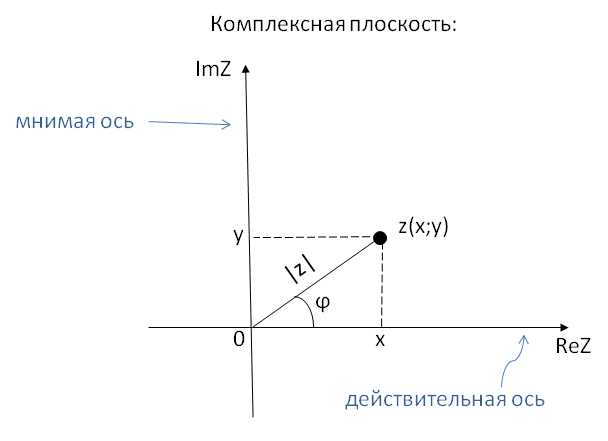
\includegraphics[scale=0.4]{complexplane1}

\[z = |z|(\cos  \varphi + i \sin  \varphi)\]
\[|z| = \sqrt{Re^2(z) + Im^2(z)} = \sqrt{x^2 + y^2}\]

Угол, который радиус-вектор образует с положительной осью $Re(z)$
называют аргументом $z$.

\[ \varphi = \textnormal{Arg}(z)\]
\[
    \begin{cases}
        \cos  \varphi = \frac{Re(z)}{|z|} \\
        \sin  \varphi = \frac{Im(z)}{|z|}
    \end{cases}
\]

При этом $ \varphi \in (-\pi; \pi]$ называют главным значением аргумента и обозначают $\arg z$
\[Arg(z) = \arg z + 2 \pi k, k \in \mathbb{Z}\]

\parspace

\underline{\textbf{Замечание}}

\begin{enumerate}
    \item Очевидно, $|Re(z)| \le |z|; |Im(z)| \le |z|$
    \item $|z|^2 = x^2 + y^2 = (x + iy)(x - iy) = z * \overline{z}$
    \item Из связи прямоугольной и полярной системы координат 
    
    $\implies Re(z) = |z| \cos (Arg(z)), Im(z) = |z| \sin (Arg(z)) \\
    z = Re(z) + i*Im(z) = |z|(\cos  \varphi + i \sin  \varphi)$ -- \textbf{тригонометрическая
    форма записи комплексного числа}.
\end{enumerate}

\subsection{Показательная форма записи комплексного числа}

Рассмотрим функцию Эйлера: $e^{i  \varphi} = \cos  \varphi + i \sin  \varphi$

\begin{theorem}[Свойства функции Эйлера]
    \begin{enumerate}
        \item $e^{i  \varphi_1} * e^{i  \varphi_2} = e^{i( \varphi_1 +  \varphi_2)}$
        \item $\frac{e^{i  \varphi_1}}{e^{i  \varphi_2}} = e^{i( \varphi_1 -  \varphi_2)}$
        \item $(e^{i  \varphi})^n = e^{i n  \varphi} \quad (n \in \mathbb{N})$
    \end{enumerate}    
\end{theorem}

\begin{proof}
    \begin{enumerate}
        \item
        \item
        \item
    \end{enumerate}    
\end{proof}

Введя функцию Эйлера: $z = |z| (\cos \varphi + i \sin \varphi), \quad z = |z| e^{i \varphi}$

\underline{\textbf{Замечание:}}

\begin{align*}
    z_1 &= |z_1| e^{i \varphi_1} \quad \varphi_1 = \textnormal{Arg} z i \\
    z_2 &= |z_2| e^{i \varphi_2} \\
    z_1 * z_2 &= |z_1| |z_2| e^{i (\varphi_1 + \varphi_2)} \\
    \frac{z_1}{z_2} &= \frac{|z_1|}{|z_2|} e^{i (\varphi_1 - \varphi_2)}, \, z_2 \ne 0 \\
    \textnormal{Arg} (z_1 * z_2) &= \textnormal{Arg} z_1 + \textnormal{Arg} z_2 \\
    \textnormal{Arg} (\frac{z_1}{z_2}) &= \textnormal{Arg} z_1 - \textnormal{Arg} z_2 \\
    \textnormal{Хотя } \textnormal{arg} (z_1 * z_2) &= \textnormal{Arg} z_1 + \textnormal{Arg} z_2 \textnormal{ не всегда}
\end{align*}

\underline{\textbf{Свойства $|z|$:}}

\begin{enumerate}
    \item $|z| \ge 0$
    \item $|z_1 * z_2| = |z_1| * |z_2|$
    
    $\left| \frac{z_1}{z_2} \right| = \frac{|z_1|}{|z_2|} \quad (z_2 \ne 0)$

    \item Неравенство $\triangle$
    
    $\left| |z_1| - |z_2| \right| \le |z_1 \pm z_2| \le |z_1| + |z_2|$
    
    $|z_1 \pm z_2|^2 = (z_1 \pm z_2) * \overline{(z_1 \pm z_2)} 
    = (z_1 \pm z_2) (\overline{z_1} \pm \overline{z_2})
    = z_1 * \overline{z_1} + z_2 * \overline{z_2} \pm (z_2 * \overline{z_2} + z_1 * \overline{z_1})
    = |z_1|^2+|z_2|^2 \pm 2 \real (z_2 * \overline{z_1})$

    $\real (z_2 * \overline{z_1}) \le |z_2 * \overline{z_1}| = |z_2| |\overline{z_1}| = |z_1| * |z_2|$

    $(|z_1|-|z_2|)^2 \le |z_1 \pm z_2| \le (|z_1| + |z_2|)^2
    = | |z_1| - |z_2| | \le |z_1 \pm z_2| \le |z_1| + |z_2|$
\end{enumerate}

